\documentclass{ctexart}
\usepackage{PhysicalChemistryNote}

\begin{document}\pagestyle{plain}
\noindent\tbf{\LARGE 6E 电解与极化作用}\vspace{15pt}\\
\indent 我们在前面主要讨论了原电池,而并没有涉及化学电池中另一重要的类别——电解池.%
理论上,只需给电池外加大于其电动势的电压,就能使其变为电解池,而实际操作中往往要外加比理论值大得多的电压.%
这是由于电极的计划作用所致.本节,我们就来详细讨论电解池以及极化作用的原理.\vspace{12pt}\\
\Section{6E.1 分解电压与极化作用}
\Part{分解电压}
\indent 我们以\ce{Pt}电极电解\ce{HCl}水溶液为例.调节施加的电压$U$,测定对应的电流$I$,得到电解时的$U-I$曲线,如下图所示.
\begin{figure}[H]
    \centering\documentclass{standalone}
\usepackage{PhysicalChemistryNote}
\begin{document}
\begin{tikzpicture}
    \draw[-latex] (0,0)--(5,0) node[right] {$U$};
    \draw[-latex] (0,0)--(0,5) node[left] {$I$};
    \draw[thick,blue,domain=0:2.5] plot[smooth] (\x,{\x^2/4});
    \draw[thick,blue,domain=2.5:5] plot[smooth] (\x,{1.25*\x-1.25*1.25});
    \draw[dashed,domain=1.25:2.5] plot[smooth] (\x,{1.25*\x-1.25*1.25});
    \node[below] at (1.25,0) {$E_{\text{b},\max}$};
\end{tikzpicture}
\end{document}
\end{figure}
开始施加外电压时,尚没有\ce{H2}与\ce{Cl2}生成.继续增大外电压,在电极上开始有\ce{H2}与\ce{Cl2}生成,%
并形成与外加电压方向相反的原电池,从而形成\tbf{反电动势}.
\begin{definition}[6E.1.1 反电动势]
    电解时,电解产物附着在电极上产生的与外加电压方向相反的电势差$E_\text{b}$称为\tbf{反电动势}.
\end{definition}
在产生气体的初期,电极上生成的\ce{H2}和\ce{Cl2}会由于浓度太低而直接向溶液扩散.%
只有当电压达到一定值时,\ce{H2}和\ce{Cl2}的分压增大到与大气压相等,反电动势$E_{\text b}$达到最大值$E_{\text b,\max}$%
(\ce{H2}和\ce{Cl2}的分压至多与大气压相等),然后\ce{H2}和\ce{Cl2}就会从溶液中逸出.此后,电流满足欧姆定律,有
\[U-E_{\text b,\max}=IR\]
因此电流$I$与外加电压$U$呈线性关系.由此不难知道,将$U-I$图线的直线部分反向延长后与$U$轴的交点即为$E_{\text b,\max}$.
\begin{hint}
    实际上,上面的$E-I$图没有十分精确的理论意义,由图得出的分解电压也并不十分精确,%
    实验的重现性也并不好,但这一实验仍有相当的价值.
\end{hint}
\begin{definition}[6E.1.2 分解电压]
    使给定电解过程连续稳定进行所必须施加的最小外加电压称为\tbf{分解电压},即上文所说的$E_{\text b,\max}$.
\end{definition}
理论上,分解电压应当等于对应的原电池的可逆电动势$E_{\text{rev}}$%.
然而,实验表明,用\ce{Pt}电极电解几种酸或碱的溶液(产物为\ce{H2}和\ce{O2}),分解电压都在$1.7\V$左右,%
这远高于理论电动势$1.23\V$.这也表明实际过程是在不可逆的条件下进行的.%
我们在下一小节就将讨论这一现象产生的原因.\vspace{4pt}\\
\Part{极化与超电势}
\indent 我们已经知道分解电压总是与理论的可逆电动势有差异.这是由于\tbf{电极的极化}所致.
\begin{definition}[6E.1.3 极化]
    在有电流通过时,电极的电势对理论值的偏离称作\tbf{极化}作用.
\end{definition}
为了定量地描述极化现象,我们将电极电势的实际值对理论值的偏离称作\tbf{超电势}.
\begin{definition}[6E.1.4 超电势]
    把某一电流密度下电极的实际电势$\varphi_{\text{re}}$与理论电势$\varphi_{\text{id}}$之差称作电极的\tbf{超电势},记作$\eta$.
\end{definition}
一般而言,电极的极化作用主要是由浓差极化和电化学极化造成的,%
超电势也主要由这两种效应贡献.我们先来讨论浓差极化.\\
\indent \tbf{浓差极化}主要是电解时电极附近溶液和其余部分(远离电极的部分)浓度不同导致的.%
例如,用\ce{Cu}电极电解\ce{CuCl2}溶液时,%
在阴极消耗\ce{Cu^2+}的速率如果快于\ce{Cu^2+}向阴极迁移的速度,%
那么电极附近的\ce{Cu^2+}浓度就将降低,从而与远处的溶液形成电势差.
\begin{definition}[6E.1.5 浓差极化]
    \tbf{浓差极化}是指电极反应足够快速使得电极附近反应物浓度低,与溶液本体产生明显浓度差异而导致电极电位偏离平衡电位的现象.
\end{definition}
\begin{hint}
    从定义上说,浓差极化\tbf{6C.3.1}的双电层是不同的概念.%
    但似乎一些教材认为剧烈搅拌可以削弱扩散层从而减少浓差极化.%
    总之,这两个概念有一定相似性,但笔者认为你还是清楚地知道两者应用的场景%
    (浓差极化出现在电解过程中,双电层出现在电极与溶液平衡时).
\end{hint}
尽管理论上,只要外加电压大于电池理论的电动势即可发生电解反应,但即使在搅拌得十分完全的情形下也很难做到如此.%
我们总是需要更高的电压使得电解顺利进行(这在气体参与的电极反应中尤为明显),%
这主要是由于电极反应大多是分步进行的,如果某一步反应的电子得失不够徐速,就会导致整个反应在电极表面受阻,%
从而使得电极电势偏离理论电势.%
我们把这一现象称为\tbf{电化学极化}.
\begin{definition}[6E.1.6 电化学极化]
    \tbf{电化学极化}是指由于电化学反应过程中电子得失不够快速,反应在电极表面受阻而导致电极电位偏离平衡电位的现象.
\end{definition}
因此,电化学极化实际上与我们将在\tbf{Chapter 7}中讲到的化学反应动力学有密切的联系.\vspace{12pt}\\
\Section{6E.2 电极反应动力学}
\Part{Butler-Volmer方程\footnote{本小节内容不必掌握,仅作参考.作为提示,你可以在学习\tbf{Chapter 7}后再来学习此方程的推导.}}
\indent 根据基本的电化学知识和化学动力学知识,我们可以推导出超电势$\eta$与电流密度$i$之间的关系.
\begin{derivation}
    我们从最简单的单电子氧化还原反应开始.考虑反应
    \begin{tightcenter}
        \ce{Ox + e^- <=>T[$k_f$][$k_b$] Red}
    \end{tightcenter}
    依照过渡态理论,我们可以简单地把这一过程的能量(如果你与读了前面的电化学势一节,就会知道这里的能量事实上指电化学势能)曲线与反应坐标的关系表示如下.
    \begin{center}
        \documentclass{standalone}
\usepackage{PhysicalChemistryNote}
\begin{document}
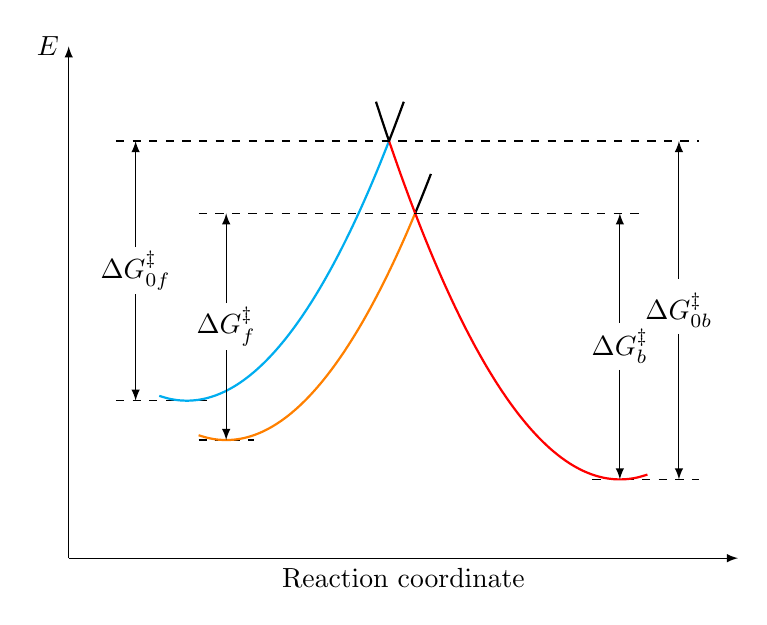
\begin{tikzpicture}
    \draw[-latex] (-1,0)--(7.5,0);
    \node[below] at (3.25,0) {Reaction coordinate};
    \draw[-latex] (-1,0)--(-1,6.5) node[left] {$E$};
    \draw[dashed] (-0.4,2)--(0.85,2);
    \draw[dashed] (0.65,1.5)--(1.35,1.5);
    \draw[dashed] (5.65,1)--(7,1);
    \draw[thick,cyan,domain=0.15:3.068] plot[smooth] (\x,{(\x-0.5)^2/2+2});
    \draw[thick,domain=3.068:3.2557] plot[smooth] (\x,{(\x-0.5)^2/2+2});
    \draw[thick,orange,domain=0.65:3.4] plot[smooth] (\x,{(\x-1)^2/2+1.5});
    \draw[thick,domain=3.4:3.6] plot[smooth] (\x,{(\x-1)^2/2+1.5});
    \draw[thick,red,domain=3.068:6.35] plot[smooth] (\x,{(\x-6)^2/2+1});
    \draw[thick,domain=2.9026:3.068] plot[smooth] (\x,{(\x-6)^2/2+1});
    \draw[dashed] (-0.4,5.29777)--(7,5.29777);
    \draw[dashed] (0.65,4.38)--(6.25,4.38);
    \node at (-0.15,3.6488) {$\Delta G^\ddagger_{0f}$};
    \draw[-latex] (-0.15,3.9488)--(-0.15,5.2977);
    \draw[-latex] (-0.15,3.3488)--(-0.15,2);
    \node at (1,2.94) {$\Delta G^\ddagger_{f}$};
    \draw[-latex] (1,3.24)--(1,4.38);
    \draw[-latex] (1,2.64)--(1,1.5);
    \node at (6.75,3.1488) {$\Delta G^\ddagger_{0b}$};
    \draw[-latex] (6.75,3.5488)--(6.75,5.2977);
    \draw[-latex] (6.75,2.8488)--(6.75,1);
    \node at (6,2.69) {$\Delta G^\ddagger_{b}$};
    \draw[-latex] (6,2.99)--(6,4.38);
    \draw[-latex] (6,2.39)--(6,1);
\end{tikzpicture}
\end{document}
    \end{center}
    其中蓝线为理论电势(这里的理论电势是\ce{Ox}和\ce{Red}浓度一定时的理论电极电势,并非标准状态对应的电极电势.)下\ce{Ox}与\ce{e^-}的能量,%
    橙线为实际电解的电势下\ce{Ox}与\ce{e^-}的能量.%
    显然,在理论电势下,反应的历程为蓝线-红线,而在实际电势下,反应的历程为橙线-红线.\\
    我们可以将\ce{e^-}的电势能并入自由能一项,并用处理一般体系的动力学方法处理此体系.\\
    现在将临近过渡态的区域放大,得到下图.
    \begin{center}
        \documentclass{standalone}
\usepackage{PhysicalChemistryNote}
\begin{document}
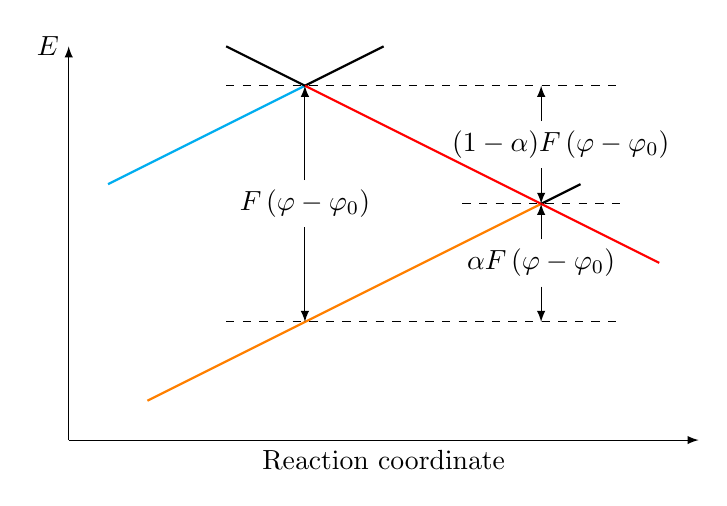
\begin{tikzpicture}
    \draw[-latex] (0,0)--(8,0);
    \node[below] at (4,0) {Reaction coordinate};
    \draw[-latex] (0,0)--(0,5) node[left] {$E$};
    \draw[thick,cyan,domain=0.5:3] plot[smooth] (\x,{0.5*\x+3});
    \draw[thick,domain=3:4] plot[smooth] (\x,{0.5*\x+3});
    \draw[thick,orange,domain=1:6] plot[smooth] (\x,{0.5*\x});
    \draw[thick,domain=6:6.5] plot[smooth] (\x,{0.5*\x});
    \draw[thick,red,domain=3:7.5] plot[smooth] (\x,{-0.5*\x+6});
    \draw[thick,domain=2:3] plot[smooth] (\x,{-0.5*\x+6});
    \draw[dashed] (2,4.5)--(7,4.5);
    \draw[dashed] (5,3)--(7,3);
    \draw[dashed] (2,1.5)--(7,1.5);
    \node at (3,3) {$F\left(\varphi-\varphi_0\right)$};
    \draw[-latex] (3,3.3)--(3,4.5);
    \draw[-latex] (3,2.7)--(3,1.5);
    \node at (6,2.25) {$\alpha F\left(\varphi-\varphi_0\right)$};
    \draw[-latex] (6,2.55)--(6,3);
    \draw[-latex] (6,1.95)--(6,1.5);
    \node at (6.25,3.75) {$(1-\alpha)F\left(\varphi-\varphi_0\right)$};
    \draw[-latex] (6,4.05)--(6,4.5);
    \draw[-latex] (6,3.45)--(6,3);
    
\end{tikzpicture}
\end{document}
    \end{center}
    在电势为$\varphi_0$和电势为$\varphi$时的,每摩尔电子的能量差为
    \[E_{\varphi_0}-E_{\varphi}=\NA\cdot(-\e)\Delta\varphi=F\left(\varphi-\varphi_0\right)\]
    从上图中可以发现即使反应物的能量降低了$F\left(\varphi-\varphi_0\right)$,活化能却并不降低相同的值.%
    定义\tbf{转移系数}$\alpha$衡量活化能附近反应物和生成物在过渡态附近的斜率(我们将在后面提到其真正的物理定义).%
    当两边斜率相同时,$\alpha=\dfrac12$.%
    这一系数也被称为\tbf{对称因子}.因此,根据Eyring方程有
    \[k_{f0}=A_f\exp\left(-\dfrac{\Delta G_{0f}^\ddagger}{RT}\right)\]
    \[k_{b0}=A_b\exp\left(-\dfrac{\Delta G_{0b}^\ddagger}{RT}\right)\]
    其中$A_f,A_b$分别为两个反应的指前因子.我们认为指前因子不随电势发生变化.\\
    考虑两张图中不同电势下正逆反应的活化能的差值,有
    \[\Delta G_{f}^\ddagger=\Delta G_{0f}^\ddagger+F\left(\varphi-\varphi_0\right)-(1-\alpha)F\left(\varphi-\varphi_0\right)
    =\Delta G_{0f}^\ddagger+\alpha F\left(\varphi-\varphi_0\right)\]
    \[\Delta G_{b}^\ddagger=\Delta G_{0b}^\ddagger-(1-\alpha)F\left(\varphi-\varphi_0\right)\]
    于是再根据Eyring方程有
    \[k_f=A_f\exp\left(-\dfrac{\Delta G_{0f}^\ddagger}{RT}\right)\exp\left(-\dfrac{\alpha F\left(\varphi-\varphi_0\right)}{RT}\right)
    =k_{f0}\exp\left(-\dfrac{\alpha F\left(\varphi-\varphi_0\right)}{RT}\right)\]
    \[k_b=A_f\exp\left(-\dfrac{\Delta G_{0b}^\ddagger}{RT}\right)\exp\left(\dfrac{(1-\alpha)F\left(\varphi-\varphi_0\right)}{RT}\right)
    =k_{b0}\exp\left(\dfrac{(1-\alpha)F\left(\varphi-\varphi_0\right)}{RT}\right)\]
    理想情况下,在\ce{Ox}和\ce{Red}浓度一定时,如果$\varphi=\varphi_0$,则电极反应达到平衡,此时有
    \[k_{f0}c_{\ce{Ox}}=k_{b0}c_{\ce{Red}}\]
    由于电极反应发生在电极的表面上,因此反应速率应当正比于电极的表面积.因此,这里的速率是指单位面积上的反应速率,速率常数$k_f$和$k_b$亦如此.%
    在此时,尽管净电流为$0$,但电子的转移仍在电极上发生,其电流密度
    \[j_0=\dfrac{I_0}{A}=\dfrac{F\Delta n_{\e^-,0}}{At}=F\dfrac{v_{\text{eq}}}{A}=Fk_{f0}c_{\ce{Ox}}=Fk_{b0}c_{\ce{Red}}\]
    这样,实际的电流密度即为
    \[\begin{aligned}
        j
        &= \dfrac{I}{A}=\dfrac{F\Delta n_{\ce{e^-}}}{At}=F\left(k_fc_{\ce{Ox}}-k_bc_{\ce{Red}}\right) \\
        &= F\left[k_{f0}c_{\ce{Ox}}\exp\left(-\dfrac{\alpha F\left(\varphi-\varphi_0\right)}{RT}\right)-k_{b0}c_{\ce{Red}}\exp\left(\dfrac{(1-\alpha)F\left(\varphi-\varphi_0\right)}{RT}\right)\right] \\
        &= j_0\left[\exp\left(-\dfrac{\alpha F\left(\varphi-\varphi_0\right)}{RT}\right)-\exp\left(\dfrac{(1-\alpha)F\left(\varphi-\varphi_0\right)}{RT}\right)\right]
    \end{aligned}\]
    而$\varphi-\varphi_0$就是我们定义的超电势$\eta$,因此上式即
    \[j=j_0\left[\exp\left(-\dfrac{\alpha F\eta}{RT}\right)-\exp\left(\dfrac{(1-\alpha)F\eta}{RT}\right)\right]\]
    这就是电极反应动力学中一个重要的方程——Butler-Volmer方程.
\end{derivation}
以上的结论都是在忽略浓差极化时推得的.由此,就有
\begin{theorem}[6E.2.1 Butler-Volmer方程]
    在参与电极反应的物质的浓度一定时,电极的电流密度$j$与超电势$\eta$满足
    \[j=j_0\left[\exp\left(-\dfrac{\alpha F\eta}{RT}\right)-\exp\left(\dfrac{(1-\alpha)F\eta}{RT}\right)\right]\]
    其中$j_0$为\tbf{交换电流密度},即电极反应平衡时的电流密度.$\alpha$为\tbf{转移系数},其物理意义将在下面进一步说明.
\end{theorem}
转移系数的物理定义如下.
\begin{definition}[6E.2.2 转移系数]
    \tbf{转移系数}$\alpha$,定义为还原反应活化能$\Delta G_{f}^\ddagger$对电势$\varphi$在$\varphi=\varphi_0$处的偏导数与Faraday常数之比的负值,即
    \[\alpha=-\dfrac{1}{F}\left.\left(\dfrac{\p\Delta G_{f}^\ddagger}{\p\varphi}\right)\right|_{\varphi=\varphi_0}\]

\end{definition}
转移系数的几何意义已经在前面的推导与图示中说明了.对于一般的反应,$\alpha$在$0.3$到$0.7$左右.\\
\indent 当超电势$\eta\to0$时,根据近似$\e^x\sim 1+x$,可将\tbf{6E.2.1}简化为
\[j=-\dfrac{j_0\alpha F\alpha}{RT}\]
这里的负号是由于超电势$\eta>0$时将发生与原电池电流方向相反的电解过程,因此令此时的电流密度为负值.这也可以由前面的推导看出.\vspace{4pt}\\
\Part{Tafel公式\footnote{Tafel公式是应当记忆的结论,但是其推导则如前面一样也不做要求.}}
\indent 1905年,Tafel研究氢电极的超电势,得出了Tafel公式.
\begin{theorem}[6E.2.3 Tafel公式]
    超电势$\eta$与电流密度$j$满足
    \[\eta=a+b\ln j\]
    其中$a$和$b$在一定温度下为常数.
\end{theorem}
这也可以由Butler-Volmer方程近似得到.
\begin{proof}
    首先需要注意的是,氢电极在电解时作为阴极,其超电势$\eta$为负值(有时也用$\eta_{\text{Cat}}$表示).%
    对于Butler-Volmer方程,当$\eta$是较大的负值时,可以将第二项忽略,从而有
    \[j=j_0\exp\left(-\dfrac{\alpha F\eta}{RT}\right)\]
    两边取对数可得
    \[\ln j=\ln j_0-\dfrac{\alpha F\eta}{RT}\]
    于是
    \[-\eta=-\dfrac{RT}{\alpha F}\ln j_0+\dfrac{RT}{\alpha F}\ln j\]
    令
    \[a=-\dfrac{RT}{\alpha F}\ln j_0\ \ \ \ \ b=\dfrac{RT}{\alpha F}\]
    即可得到Tafel公式.由于$\alpha$的值一般在$0.5$左右,因此$b$的值在一定温度下对于各种反应相差都不大,而$a$则主要取决于具体的反应和电极类型.\\
    阳极的Tafel公式的推导也是类似的,在这里就不再赘述了.
\end{proof}
我们再一次声明,以上的结论都是在忽略浓差极化时推得的.%
对于反应迅速的反应过程,大过电位下将直接到达浓差极化为主的阶段,%
没有明显的Tafel现象.而对于反应动力学缓慢,具有较大的活化能的反应,可以观察到很好的Tafel关系,此时逆反应几乎可以忽略,也反映了反应的完全不可逆性.%
氢电极就是这样的一种电极,Tafel公式对其符合得较好.
\end{document}